%% ----------------------------------------------------------------------------
% BIWI SA/MA thesis template
%
% Created 09/29/2006 by Andreas Ess
% Extended 13/02/2009 by Jan Lesniak - jlesniak@vision.ee.ethz.ch
%% ----------------------------------------------------------------------------

% Give an introduction to the topic you have worked on:
% 
% \begin{itemize}
%  \item \textit{What is the rationale for your work?} Give a sufficient description of the problem, e.g. with a general description of the problem setting, narrowing down to the particular problem you have been working on in your thesis. Allow the reader to understand the problem setting. 
%  \item \textit{What is the scope of your work?} Given the above background, state briefly the focus of the work, what and how you did.
%  \item \textit{How is your thesis organized?} It helps the reader to pick the interesting points by providing a small text or graph which outlines the organization of the thesis. The structure given in this document shows how the general structuring shall look like. However, you may fuse chapters or change their names according to the requirements of your thesis.
% \end{itemize}

\chapter{Introduction}
With the increase of computational power the field of computer vision has made huge leaps forward in recent years. The integration of machine learning techniques and especially the introduction of deep Convolutional Neural Networks (CNN) allowed for unparalleled performance on classification and detection tasks~\cite{krizhevsky2012}. Convolutional neural network do not only automate feature selection and classification, but also feature design which has been a complicated topic in computer vision research over the years\needref. Neural networks provide a large learning capacity and the capability to learn every type of function. However, with several milions of parameters, those networks need large labeled datasets to prevent overfitting and to learn powerful generalizable models.

Nowadays datasets like Imagenet provide millions of labeled images in over thousands of categories~\cite{deng2009}, overcoming earlier shortcomings of smaller datasets. Efforts to scale these methods to billions of images are however hampered by the expense of human annotation required~\cite{doersch2015}, limiting possibilities for improvements in the future. The costly and time-consuming process of manual annotation harms the scalability to new problem domains in particular, especially for tasks involving more complex data (like videos and 3D imaging \needref) and tasks requiring expertise~\cite{lee2017,fernando2017}. In this context it would be legitimate to ask: do we really need strong-supervision from so many images to train those CNNs~\cite{wang2015}?

Unfortunately, despites decades of sustained effort, unsupervised learning have not yet reached the level to allow it to extract useful information from large collection of full-size images~\cite{doersch2015}. Humans however excel in inferring 3D structure and developing a strong belief of structure also in short timescales, while receiving only limited semantic supervision. One hypothesis of the reason humans perform so well in this task is that we develop a rich structural understanding of the world through past visual experience and creating consistent modeling of our observations~\cite{zhou2017}. In this way the context has shown to be an important factor in learning, which leads to the concept of self-supervised learning.

\begin{figure}[t]
\centering
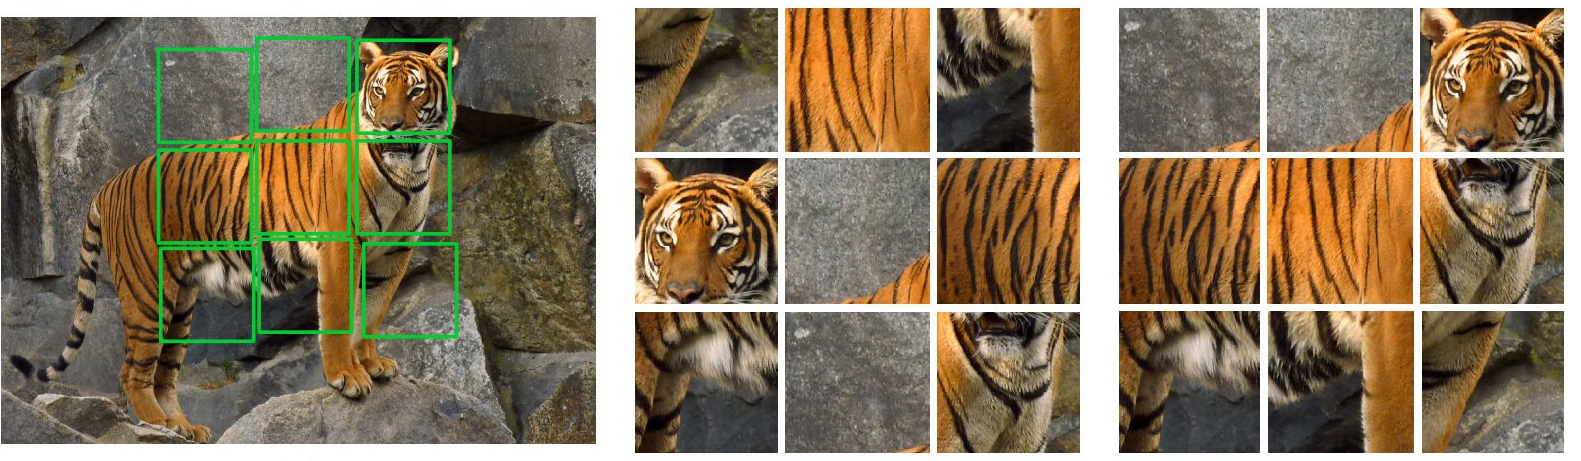
\includegraphics[width=\textwidth]{images/jigsaw_puzzle.png}
\caption{Example of a self-supervised task to let a neural network solve a jigsaw puzzle as explored by Noorozi et al\cite{noroozi2016}. Tiles (green) are extracted from the image and a puzzle is obtained by shuffling them, that is fed to the CNN to solve. Figure is reproduced from \cite{noroozi2016}.}
\label{fig:jigsaw}
\end{figure}

Self-supervised learning is the use of all the 'free' data available and exploits its intrinsic structure for training neural networks. Self-supervised learning techniques can exploit reward signals from both both spatial coherence, for example by learning the correct location of patches~\cite{doersch2015, noroozi2016} with an example in Figure \ref{fig:jigsaw}. Alternatively temporal coherence can be used, for example by learning to order frames in videos~\cite{misra2016, lee2017}. Although these tasks are rather specialized, these self-taught features can often generalize well to a certain extent. By using transfer learning the performance on supervised tasks can be improved, as the networks learn similar basic visual patterns required for object detection and classification~\cite{raina2007}. In the framework of CNNs this optimization procedure is usually referred to a 'fine-tuning', giving similar classification performance with much less supervision \needref.

Autonomous driving has recently seen a huge interest both from a commercial perspective as well as in robotics research. This topic is closely related to the field of computer vision, with detection of objects like cars, pedestrians and signs being a major part allowing to drive autonomously. The application of convolutional neural networks has achieved huge success in improving object detection \needref, but suffers again from the requirement of huge annotated datasets for sufficient performance \needref. Various datasets like the Kitti~\cite{geiger2012} and the Oxford Robotcar~\cite{maddern2017} dataset contain driving videos with cameras from various perspectives, combined with high-quality lidar measurements, precise GPS tagging and accurate timing. These datasets therefore have extensive intrinsic structure and should thus be an excellent source for self-supervised learning. 

\section{Focus of this Work}
This work tries to take advantage of the free data in driving datasets. The expensive labeling in those datasets is not used, but instead self-supervising techniques are explored to learn features. The core of this report is the use of an order-prediction task to learn the temporal coherence between lidar and camera images and experiments to validate the generalization of the features learned in such a network.

\section{Thesis Organization}
This thesis is organized in several sections. Section \ref{ch:related_work} contains a literature research to related work in self-supervised learning and the application of lidar and gps signals for learning. In Section \ref{ch:implementationdetails} the general neural network implementation, data sampling and researched variations are put forward. The performance of the neural network and the application of the learned model to other tasks are presented in Section \ref{ch:experimentsandresults}, followed by a detailed discussion in Section \ref{ch:discussion}.
